Table~\ref{tab:kv} and Fig.~\ref{fig:kv} compare the uncached reference with the two cache implementations on the same fine-tuned model and the same real prompts (validation-split prompt tokens cut to the stated length), with EOS disabled so each run emits exactly the stated number of tokens (one warm-up, two timed runs, median reported).

\textbf{Token agreement.} For all four input/output settings with a reference (64/32, 256/32, 512/32, 128/64) the cached greedy tokens are \emph{identical} to the uncached ones, and the pre-allocated and concatenating caches agree with each other in all six settings. Unit tests extend this to three further lengths on the 135M model, to the tiled attention backend, to chunked prefill (a prompt fed in three pieces gives the same logits as one pass, $<10^{-4}$) and to cache cropping followed by re-feeding (the operation speculative decoding relies on). The benchmark logs the top-2 logit margin at the first divergent position if a mismatch occurs; none occurred, consistent with fp32 logit differences of $\sim10^{-5}$ being far smaller than typical greedy margins.

\begin{table*}[t]\centering\caption{KV-cache benchmark, fine-tuned SmolLM2-360M, fp32, 10 CPU threads. Times in seconds (median of 2 after warm-up); KV MB is the analytic fp32 cache size ($80$\,KiB/token); $\Delta$RSS is peak resident-memory increase (KV / no-cache).}\label{tab:kv}
\begin{tabular}{rrrrrrrrrrrl}\toprule
In & Out & No-cache & KV static & KV concat & KV prefill & KV decode & KV dec.\ tok/s & No-cache tok/s & KV MB & $\Delta$RSS MB & Same tokens\\\midrule
64 & 32 & 15.17 & 5.12 & 5.26 & 0.289 & 4.37 & 7.1 & 2.1 & 7.5 & 9/6 & yes \\
256 & 32 & 40.76 & 5.42 & 5.73 & 0.800 & 4.86 & 6.4 & 0.8 & 22.5 & 30/5 & yes \\
512 & 32 & 93.80 & 7.46 & 7.52 & 1.633 & 6.18 & 5.0 & 0.3 & 42.5 & 11/12 & yes \\
128 & 64 & 85.93 & 19.45 & 19.49 & 1.240 & 18.35 & 3.4 & 0.7 & 15.0 & 9/39 & yes \\
1024 & 64 & -- & 30.25 & 28.80 & 7.725 & 21.76 & 2.9 & -- & 85.0 & 761/-- & n/a \\
2048 & 32 & -- & 30.83 & 29.22 & 18.953 & 13.92 & 2.2 & -- & 162.5 & 97/-- & n/a \\
\bottomrule\end{tabular}\end{table*}

\begin{figure}[t]\centering
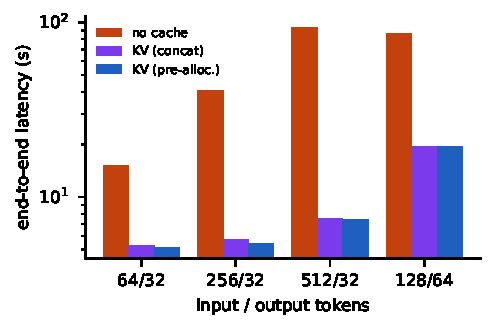
\includegraphics[width=\columnwidth]{figures/kv_latency.pdf}
\caption{End-to-end greedy generation latency (log scale) without cache, with a concatenating cache and with the pre-allocated cache.}\label{fig:kv}
\end{figure}

\textbf{Speed.} The cache turns each decode step from a forward pass over the whole sequence into a single-token pass, so the speed-up grows with context: 3.0$\times$ at 64 input tokens, 7.5$\times$ at 256 and \kvMaxSpeedup$\times$ at 512 (32 new tokens). Without a cache, throughput collapses from 2.1 to 0.34 tokens/s as the prompt grows; with the cache, decode throughput falls only mildly (7.1$\rightarrow$5.0 tokens/s) because attention over a longer cache is cheap compared to the weight-bound MLP and projection work. A single decode step must stream all 1.45\,GB of fp32 weights from memory, so 3--7 tokens/s is close to the memory-bandwidth limit of this laptop, which is why decode---not prefill---dominates end-to-end latency for short prompts. Prefill time scales roughly linearly to super-linearly with prompt length (0.29\,s for 64 tokens, 7.7\,s for 1{,}024, 19.0\,s for 2{,}048 tokens), reflecting the quadratic attention term at long contexts.

\textbf{Memory and cache growth.} The cache costs 80\,KiB per token (7.5\,MB at 96 tokens, 162\,MB at 2{,}080 tokens), small next to the 1.45\,GB of weights for our prompt lengths but linear in context and batch size, which is why GQA (5 instead of 15 KV heads, a 3$\times$ saving) matters. The measured RSS increases are dominated by allocator behaviour and transient activations (e.g.\ 761\,MB during the 1{,}024-token prefill) and are noisy; we report them but rely on the analytic sizes. The concatenating cache re-allocates every step ($O(N^2)$ copying) yet is within a few percent of the pre-allocated one at these lengths, because copying a few tens of MB is negligible next to a 1.45\,GB weight read; the pre-allocated cache's real advantage here is $O(1)$ roll-back for speculative decoding and a fixed memory footprint.
